\chapter{Results and Analysis}
\lhead{Chapter 6. \emph{Results and Analysis}}
\label{chap.6}

This chapter presents the results of evaluating the Quantum Secure File Transfer Protocol (Q-SFTP) across multiple dimensions: handshake correctness, cryptographic security, file integrity, transfer performance, and production readiness.

\section{Handshake Verification}

\subsection{Client and Server Handshake Output}

The Q-TLS handshake was tested across localhost and cross-device configurations. Figures~\ref{fig:client_handshake} and~\ref{fig:server_handshake} show the successful execution of the four-phase handshake from client and server perspectives.

\begin{figure}[H]
    \centering
    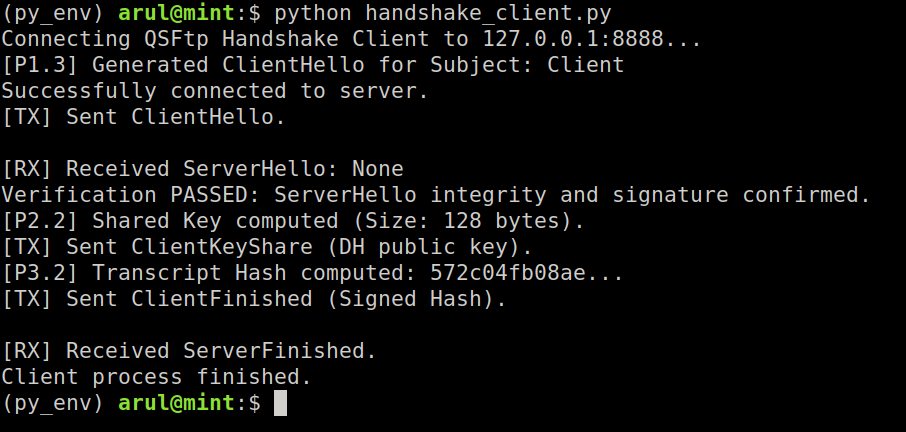
\includegraphics[width=0.9\textwidth]{Figures/client.png}
    \caption{Client-side output of the Q-TLS Handshake showing certificate verification, Kyber512 encapsulation, transcript hash computation, and session key derivation}
    \label{fig:client_handshake}
\end{figure}

\begin{figure}[H]
    \centering
    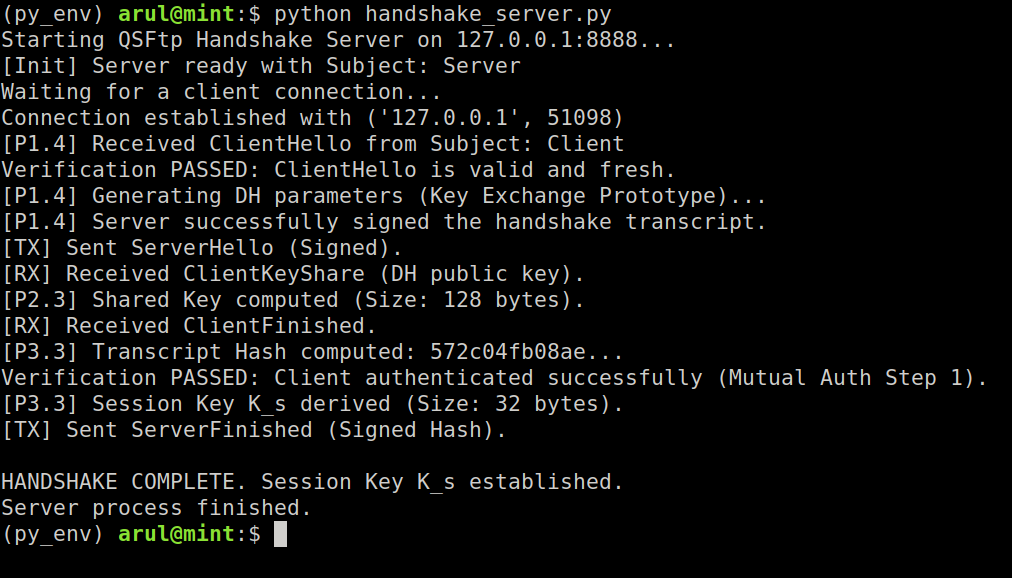
\includegraphics[width=0.9\textwidth]{Figures/server.png}
    \caption{Server-side output of the Q-TLS Handshake showing certificate validation, Kyber512 decapsulation, Dilithium2 signature verification, and session key establishment}
    \label{fig:server_handshake}
\end{figure}

The outputs confirm:
\begin{itemize}
    \item Both endpoints successfully negotiated session keys using Kyber512-based encapsulation.
    \item Mutual authentication was achieved through Dilithium2 signatures on the transcript hash.
    \item Session key derivation via HKDF-SHA256 produced identical 256-bit keys on both sides.
    \item Timestamp validation (30-second window) prevented acceptance of stale messages.
\end{itemize}

\section{Cryptographic Parameter Analysis}

Table~\ref{tab:crypto_params} summarizes the cryptographic parameters and key sizes used in Q-SFTP.

\begin{table}[H]
    \centering
    \caption{Cryptographic parameters and key sizes in Q-SFTP}
    \label{tab:crypto_params}
    \begin{tabular}{|l|c|c|c|c|}
        \hline
        \textbf{Algorithm} & \textbf{Security Level} & \textbf{Public Key} & \textbf{Secret Key} & \textbf{CT / Signature} \\
        \hline
        Kyber512 & NIST Level 1 & 800 B & 1,632 B & 768 B \\
        \hline
        Dilithium2 & NIST Level 2 & 1,312 B & 2,560 B & 2,420 B \\
        \hline
        AES-256-GCM & 128-bit (PQ) & -- & 32 B & +28 B (12 nonce + 16 tag) \\
        \hline
        BLAKE2b-256 & 128-bit (PQ) & -- & -- & 32 B \\
        \hline
    \end{tabular}
\end{table}

\begin{table}[H]
    \centering
    \caption{Dilithium Performance Benchmarks}
    \vspace{2pt}
    \label{tab:dilithium_benchmarks}
    \begin{tabular}{|l|c|c|c|}
        \hline
        \textbf{Operation} & \textbf{Dilithium2} & \textbf{Dilithium3} & \textbf{Dilithium5} \\
        \hline
        KeyGen() & 6 ms & 9 ms & 15 ms \\
        \hline
        Sign() & 27 ms & 46 ms & 58 ms \\
        \hline
        Verify() & 7 ms & 11 ms & 18 ms \\
        \hline
    \end{tabular}
    \vspace{2pt}
    % \small{\textit{\n Hardware: Intel Core i7-9750H CPU}}
\end{table}

\begin{table}[H]
    \centering
    \caption{Kyber Performance Benchmarks}
    \label{tab:kyber_benchmarks}
    \begin{tabular}{|l|c|c|c|c|c|c|}
        \hline
        \textbf{Params} & \textbf{keygen} & \textbf{keygen/s} & \textbf{encap} & \textbf{encap/s} & \textbf{decap} & \textbf{decap/s} \\
        \hline
        Kyber512 & 2.02 ms & 493.99 & 2.84 ms & 352.53 & 4.12 ms & 242.82 \\
        \hline
        Kyber768 & 3.40 ms & 294.13 & 4.38 ms & 228.41 & 6.06 ms & 165.13 \\
        \hline
        Kyber1024 & 5.09 ms & 196.61 & 6.22 ms & 160.72 & 8.29 ms & 120.68 \\
        \hline
    \end{tabular}
    \vspace{2pt}
    % \small{\textit{Hardware: Intel Core i7-9750H CPU}}
\end{table}

\section{Security Testing}

Security testing was performed using automated test scripts and manual verification. The \textbf{pytest} framework was used to validate protocol correctness and cryptographic integrity.

\subsection{Pytest Results for Q-TLS Handshake}

Figure~\ref{fig:pytest_handshake} shows the successful execution of the handshake test suite. All test cases — including certificate exchange, key encapsulation, mutual authentication, and session key derivation — passed.

\begin{figure}[H]
    \centering
    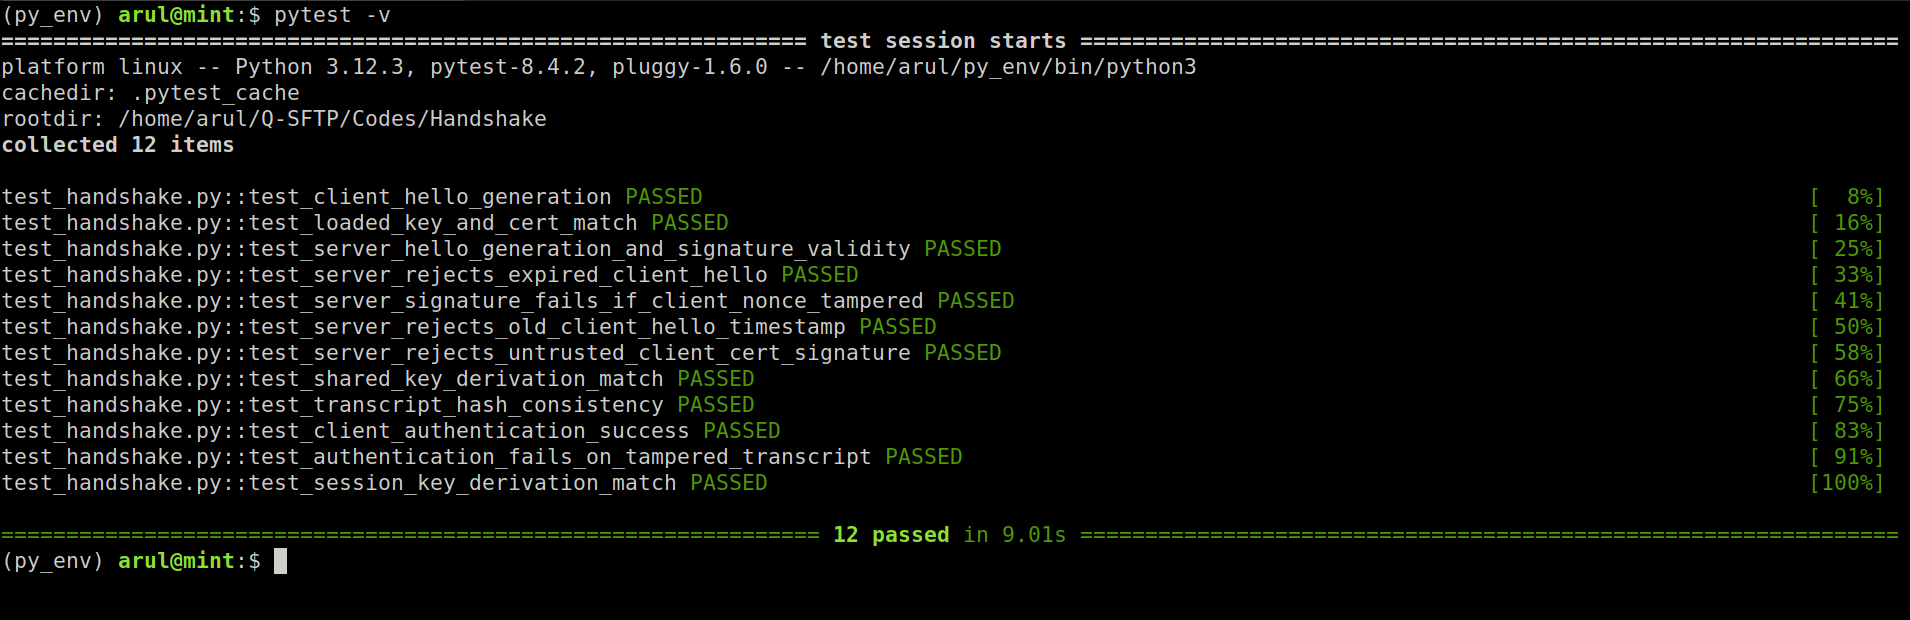
\includegraphics[width=0.9\textwidth]{Figures/pytest_handshake.png}
    \caption{Pytest Results for Q-TLS Handshake Validation}
    \label{fig:pytest_handshake}
\end{figure}

\subsection{CA Tool Testing}

The Certificate Authority module was tested separately to ensure accurate certificate issuance and Dilithium2 signature verification. Figure~\ref{fig:pytest_ca} illustrates the results.

\begin{figure}[H]
    \centering
    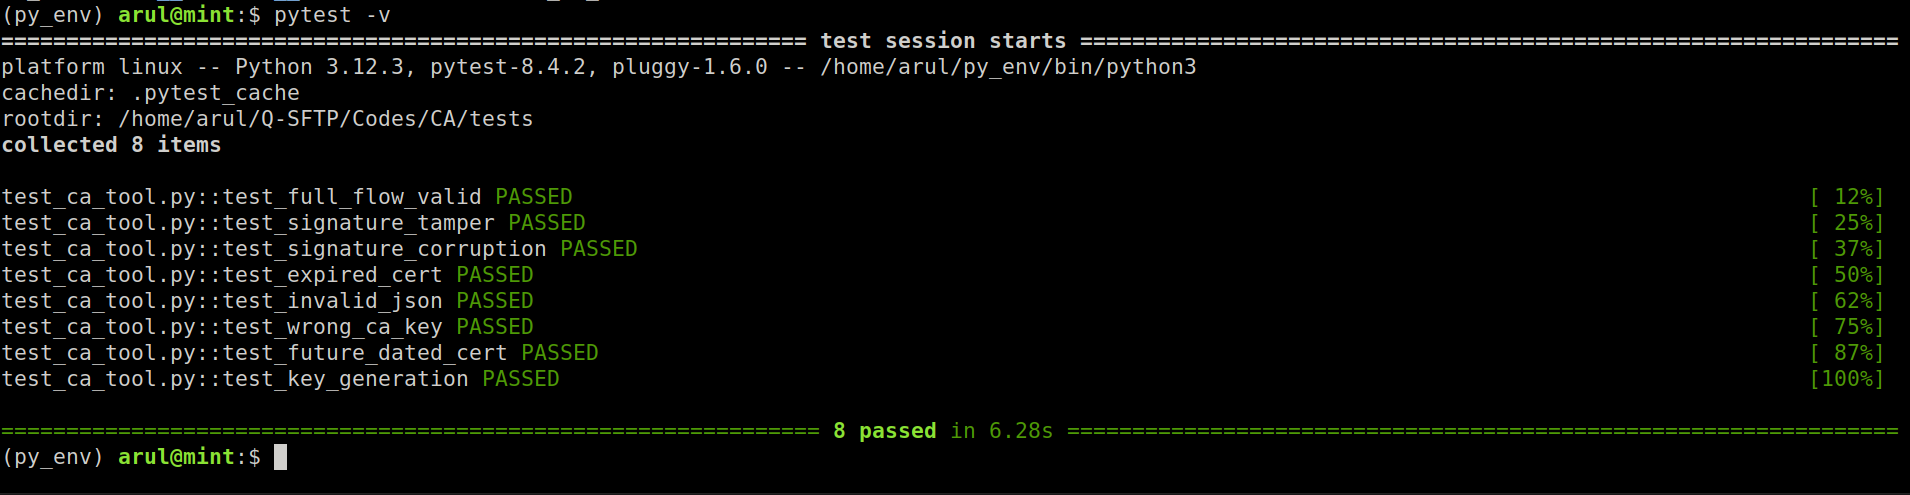
\includegraphics[width=0.9\textwidth]{Figures/pytest_ca.png}
    \caption{Pytest Results for Certificate Authority (CA) Module}
    \label{fig:pytest_ca}
\end{figure}

\subsection{File Integrity Testing (BLAKE2b)}

The BLAKE2b hash verification system was tested in four phases:

\begin{enumerate}
    \item \textbf{Phase 1 — Registration:} Files uploaded via the web interface are automatically hashed with BLAKE2b-256 and registered in \texttt{hash\_registry.json}. All test files were correctly registered with matching client-side and server-side hashes.
    
    \item \textbf{Phase 2 — Verification:} Retrieved files were re-hashed and compared against stored values. All files returned \texttt{VERIFIED} status.
    
    \item \textbf{Phase 3 — Tamper Detection:} Files were manually modified on the server. The integrity checker correctly detected mismatches and returned \texttt{TAMPERED} status with detailed reports.
    
    \item \textbf{Phase 4 — Background Monitoring:} The periodic background checker (running at configurable intervals) correctly identified both verified and tampered files during long-running tests.
\end{enumerate}

\section{Transfer Performance}

\subsection{Chunked Transfer Overhead}

The chunked transfer protocol introduces minimal overhead. For a file of size $F$ bytes with chunk size $C = 256$ KB:
\[
N_{chunks} = \left\lceil \frac{F}{C} \right\rceil
\]

Each chunk incurs an AES-256-GCM overhead of 12 bytes (nonce) + 16 bytes (tag) = 28 bytes, plus JSON message framing. For a 100 MB file:
\begin{itemize}
    \item Total chunks: $N = \lceil 100 \times 1024 \times 1024 / 262144 \rceil = 400$
    \item Cryptographic overhead: $400 \times 28 = 11,200$ bytes ($\approx 0.01\%$)
\end{itemize}

\subsection{Resume Reliability}

Resumable transfers were tested under the following conditions:
\begin{itemize}
    \item \textbf{Connection interruption:} Browser closed mid-upload, then reopened. Transfer resumed from the last confirmed chunk offset.
    \item \textbf{Page refresh:} Browser refreshed during upload. localStorage state enabled seamless resume.
    \item \textbf{Server restart:} Handshake server restarted after partial upload. Server-side \texttt{.part} file and transfer log enabled resume after re-handshake.
\end{itemize}

All three scenarios resulted in successful completion without data loss.

\section{Security Analysis}

\subsection{Quantum Resistance}
\begin{itemize}
    \item The Kyber512 key encapsulation provides IND-CCA2 security under the Module Learning With Errors (MLWE) assumption, which is believed to be hard for both classical and quantum computers.
    \item Dilithium2 provides EUF-CMA (Existential Unforgeability under Chosen Message Attack) security under MLWE and Module-SIS.
    \item AES-256-GCM maintains 128-bit security against Grover's algorithm (quadratic speedup reduces 256-bit to effective 128-bit).
\end{itemize}

\subsection{MITM Resistance}
Mutual authentication through bilateral Dilithium signatures on the transcript hash prevents man-in-the-middle attacks. An attacker would need to forge a Dilithium signature — equivalent to solving MLWE.

\subsection{Replay Attack Prevention}
\begin{itemize}
    \item Random nonces ($N_C$, $N_S$) are incorporated into key derivation.
    \item Timestamp validation rejects messages older than 30 seconds.
    \item Ephemeral Kyber key pairs provide forward secrecy per session.
\end{itemize}

\subsection{Data Integrity}
\begin{itemize}
    \item \textbf{In-transit:} AES-256-GCM authentication tags detect any modification during transmission.
    \item \textbf{At-upload:} Dual-side BLAKE2b hashing detects corruption between client and server.
    \item \textbf{At-rest:} Background integrity checker detects unauthorized server-side modifications.
\end{itemize}

\subsection{Privacy}
\begin{itemize}
    \item Metadata stripping removes identifying information from files before storage.
    \item IP anonymization via daily rotating SHA-256 salt prevents long-term tracking in audit logs.
\end{itemize}

\section{Strengths and Weaknesses}

\subsection{Strengths}
\begin{itemize}
    \item \textbf{Full quantum resistance} using NIST-standardized PQC algorithms.
    \item \textbf{Comprehensive integrity} through BLAKE2b dual-verification and background monitoring.
    \item \textbf{Resumable transfers} with persistent state on both client and server.
    \item \textbf{Privacy preservation} through automatic metadata stripping and IP anonymization.
    \item \textbf{Production-ready web interface} with admin panel and RBAC.
    \item \textbf{Modular architecture} enabling independent cryptographic upgrades.
\end{itemize}

\subsection{Weaknesses}
\begin{itemize}
    \item \textbf{Larger certificates:} PQC keys and signatures are significantly larger than classical equivalents, increasing initial handshake payload.
    \item \textbf{Computational overhead:} Kyber and Dilithium operations consume more CPU cycles than RSA/ECDH for key generation and signing.
    \item \textbf{Single-server architecture:} The current implementation does not support distributed or clustered deployment.
\end{itemize}

The results demonstrate that Q-SFTP achieves its design goals of quantum-safe integrity, confidentiality, and usability without significant performance degradation.
